\section{Parameter Learning}

\begin{frame}{Parameter Learning in SPNs}{}
\begin{columns}
\begin{column}{\linewidth}
\begin{block}{Generative Learning\footnote{\scriptsize H. Poon \& P. Domingos: Sum-product networks: A new deep architecture. In UAI, 2011.}}
\begin{equation}
  \mathcal{L}(\theta \,| \, \mathcal{X}) = \sum_{n=1}^N \log \f - \log \fz\, , \; \; \xn \in \mathbb{R}^D
\end{equation}
\end{block}
Note that $\fz$ is the partition function which can be evaluated efficiently using a single upward pass.
%\hline
\begin{block}{Discriminative Learning\footnote{\scriptsize R. Gens \& P. Domingos: Discriminative learning of sum-product networks. In NeurIPS, 2012.}}
\begin{equation}
  \begin{aligned}
    \mathcal{L}(\theta, \lambda \,| \, \mathcal{X}) = \sum_{n=1}^N &\log \fy - \log \f\, , \; \; \xn \in \mathbb{R}^D, \, \lambda_n \in \mathbb{R}
\end{aligned}
\end{equation}
\end{block}
\end{column}
\end{columns}
\end{frame}

\begin{frame}{Parameter Learning in SPNs}{}
\begin{block}{Semi-Supervised Learning using Contrastive Pessimistic Likelihood Estimation (CPLE)\footnote{\scriptsize M. Trapp et al.: Safe semi-supervised learning of sum-product networks. In UAI, 2017.}}
\begin{equation}
  \text{CPLE} = \argmax_{\theta \in \Theta} \argmin_{\bm q \in \Delta_{K-1}^M} \mathcal{L}(\theta,  \lambda, \bm{q} \,| \, \mathcal{X}, \mathcal{U}) - \mathcal{L}(\theta^+, \lambda, \bm{q} \,| \, \mathcal{X}, \mathcal{U})
\end{equation}
\end{block}

\begin{figure}
  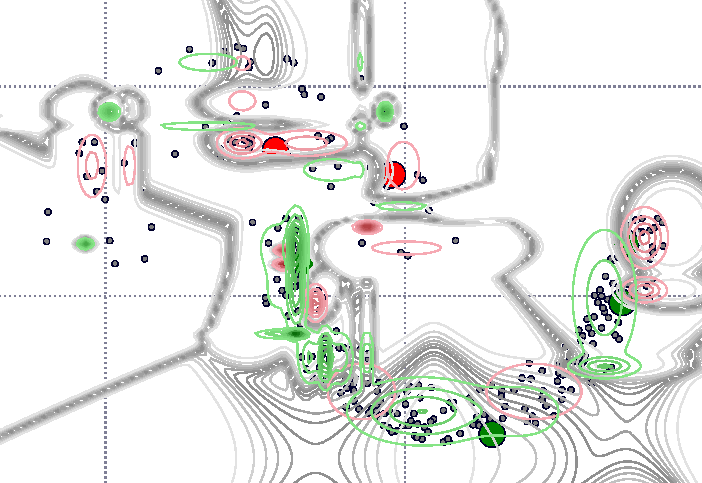
\includegraphics[width=.4\textwidth]{semisupervised_2_2}~
   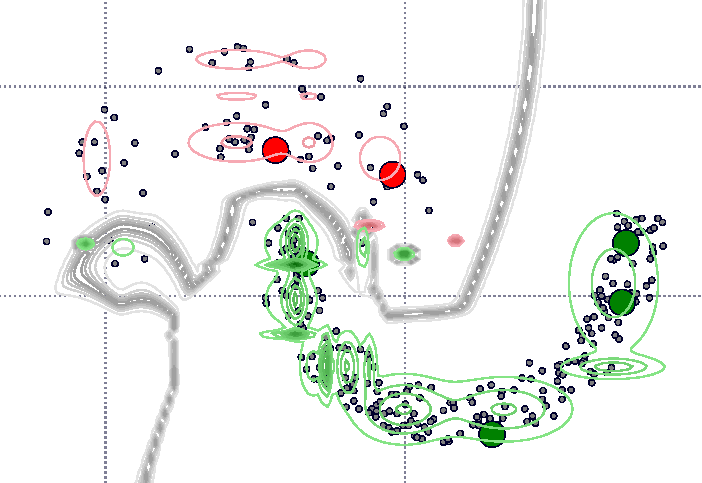
\includegraphics[width=.4\textwidth]{semisupervised_20_2}
\end{figure}

\end{frame}

\begin{frame}{Overparameterization in SPNs\footnote{\scriptsize M. Trapp et al.: Optimisation of Overparametrized Sum-Product Networks. ICML Workshop on Tractable Probabilistic Models, 2019.}}{}
\begin{columns}
\begin{column}{\linewidth}
\begin{align}
    \wt &\approx \wt + \rho^{(t)} \nabla_{\wt} + \left[ \sum_{l=0}^{L-1} \eta \nabla_{w^{[l]}_{\phi(k, l)}} (w^{[l]}_{\phi(k, l)})^{-1} \right] \wt \\
  &= \wt + {\color{cyan} \rho^{(t)}} \nabla_{\wt} + {\color{blue}\sum_{\tau=1}^{t-1} \mu^{(t,\tau)} \nabla_{w^{(\tau)}_k}}
\end{align}\\
  \begin{tcolorbox}[lower separated=false]
  \small{Gradient-based optimisation in deep tree-structured sum-product network with small (fixed) learning rate and near zero initialisation of the weights is equivalent to gradient-based optimisation with adaptive and time-varying {\color{cyan} learning rate} and {\color{blue} momentum term}.}
 \end{tcolorbox}
\end{column}
\end{columns}
\end{frame}

\iffalse
\begin{frame}{Overparameterization in SPNs \small{[Trapp 2019]}}{}
\begin{columns}
\begin{column}{\linewidth}
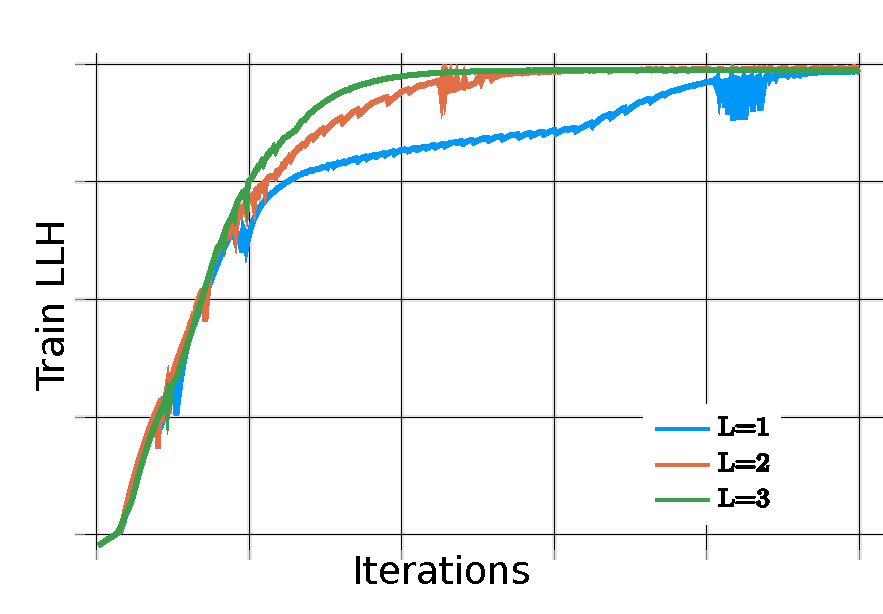
\includegraphics[width=\textwidth]{nltcs_experiment}
\end{column}
\end{columns}
\end{frame}
\fi

\iffalse
\begin{frame}{Bayesian Parameter Learning}
  \begin{itemize}
    \item The key insight for Bayesian parameter learning\footnote{\scriptsize Zhao et al.: Collapsed variational inference for sum-product networks. In ICML, 2016.}
        is that \emph{sum nodes} can be interpreted as \emph{latent variables} $Z_\SumNode$, clustering data instances.
    \item Given a vector of states for each sum, $\z$ induces a so-called induced tree ($\SPT$) on $\SPN$.
  \end{itemize}
  \begin{figure}
  \centering{
    \includestandalone[width=0.7\textwidth]{InducedTree}
    }
\end{figure}
\end{frame}
\fi

%\begin{frame}{Bayesian Parameter Learning}
%  \begin{itemize}
%    \item It is now conceptually straightforward to extend an SPN to a Bayesian setting.
%  \end{itemize}
%  \pause
%  \begin{figure}
%
%\centering
%
%\begin{tikzpicture}
%
%  \node[obs, fill=lightbackground, draw=white] (x) {$\xnd$};
%
%  \node[foreground, draw=CBYellow, latent, fill=background, left=of x] (z) {$z_{\SumNode,n}$};
%
%  \node[foreground, draw=CBPurple, latent, fill=background, right=of x] (t) {$\theta_{\Leaf,d}$};
%
%  \node[foreground, draw=CBGreen, latent, fill=background, below=of z] (w) {$w_{\SumNode}$};
%
%
%
%  \edge {z,t} {x} ; %
%
%  \edge {w} {z} ; %
%
%
%
%  \plate {zs} {(z)(w)} {$\forall \SumNode \in \SumNodes$} ;
%
%  \plate {t} {(t)} {$\forall \Leaf \in \Leaves$} ;
%
%
%
%  \plate [inner xsep=0.3cm] {xyt} {(x)(t)} {$d\!\in\!1\!:\!D$} ;
%
%  \plate [inner xsep=0.3cm] {xz} {(x)(z)(xyt.north west)} {$n\!\in\!1\!:\!N$} ;
%
%\end{tikzpicture}
%
%\caption{Generative model for Bayesian parameter learning.} \label{fig:BSPN}
%
%\end{figure}
%
%\end{frame}
